\pgfkeys{/donut/.cd,
inner radius/.initial=1cm,
inner radius=1cm,
outer radius/.initial=2.5cm,
outer radius=2.5cm,
text color/.initial=white,
text color=white}
\newcommand{\donutchart}[3][]{
   % Calculate total
   \pgfmathsetmacro{\totalnum}{0}
   \foreach [count=\n] \value/\colour/\name in {#2} {
     \pgfmathparse{\value+\totalnum}
     \global\let\totalnum=\pgfmathresult
     \xdef\numitems{\n}
   }
	\xdef\midText{#3}

  \begin{tikzpicture}
  \pgfmathsetmacro{\wheelwidth}{\pgfkeysvalueof{/donut/outer
  radius}-\pgfkeysvalueof{/donut/inner radius}}
  \pgfmathsetmacro{\midradius}{(\pgfkeysvalueof{/donut/outer radius}
  +\pgfkeysvalueof{/donut/inner radius})/2}

  \begin{scope}[#1]

    \pgfmathsetmacro{\cumnum}{0}
    \foreach \value/\colour/\name in {#2} {
        \pgfmathsetmacro{\newcumnum}{\cumnum + \value/\totalnum*360}

        \pgfmathsetmacro{\midangle}{-(\cumnum+\newcumnum)/2}
        \begin{scope}[on background layer]
          \filldraw[draw=white,fill=\colour]
          (-\cumnum:\pgfkeysvalueof{/donut/outer radius}) 
           arc(-\cumnum:-(\newcumnum):\pgfkeysvalueof{/donut/outer radius}) --
          (-\newcumnum:\pgfkeysvalueof{/donut/inner radius}) 
          arc(-\newcumnum:-(\cumnum):\pgfkeysvalueof{/donut/inner radius}) -- cycle;
        \end{scope}

			%draw
		\pgfmathparse{ifthenelse(\value < 5, 1, 0)}
		\ifnum\pgfmathresult=1
			\draw node [text=black, font=\bfseries\sffamily] at (\midangle:{\pgfkeysvalueof{/donut/inner radius}+\wheelwidth*1.2}) {\value \%};
		\else
			\draw node [text=\pgfkeysvalueof{/donut/text color}, 
			font=\bfseries\sffamily] at 
			(\midangle:{\pgfkeysvalueof{/donut/inner radius}+\wheelwidth/2}) {\value \%};
		\fi


        \global\let\cumnum=\newcumnum
    }
    
    % \node[text width=\textwidth] at (-4,0) {
    %     \foreach \value/\colour/\name in {#2} {
    %        {\color{\colour}\textbullet}\space\name \\
    %     }    
    % };
    
	\draw node [text=black, font=\bfseries\sffamily] at (0,0) {\textbf{\midText}};
    
  \end{scope}

  \end{tikzpicture}}


\section{It Is Time to Address Network Power Proportionality}
\subsection{Introduction}
In recent years, due to the growth in data centers and machine learning clusters traffic, networking hardware has prioritized throughput and performance.
This trend has led manufacturers to overlook the power efficiency of their devices at the cost of their power-to-load efficiency.

The metric used to track this power consumption to load efficiency is power proportionality. 
An ideal power proportional device would consume power in direct proportion to the work performed. 
Conversely, a non-power-proportional device would consume power near maximum regardless of the work performed. 
It is distinct from the power efficiency, as it focuses on the relation between the power and the work, whereas power efficiency focuses on the work done per power consumption.

By contrast, computing hardware has gained more attention for its power proportionality and efficiency. It is primarily due to its larger power footprint globally, as computing hardware is abundant and its idling cost, especially in large scale deployments, should stay low.

In this section, we explore an article \cite{NetPowProp} addressing such network hardware device power proportionality issues and possible solutions.
To this end, the article first tackles and models a concrete example of a machine learning cluster modeled in Section \ref{sec:PowMod}.
This scenario is somewhat of a worst case scenario to argue for network power proportionality, as the computational power demand is substantially larger than the networking one. 

However, it is observed  (Section \ref{sec:impact}) that, mainly due to the combination of poor power proportionality and low time usage, the network accounts for an average of 12\% of the total power footprint in the cluster.
This implies that in less computationally heavy environments such as data centers, the share of power consumption of the network should be a concern.   

Finally, Section \ref{sec:PowSol} explores possible improvements originating from already implemented power proportionality mechanisms from computing hardware by transposing their concepts to networking hardware.

\subsection{Modeling approach}\label{sec:PowMod}
The article analyses a production state-of-the-art machine learning cluster described in a paper from Alibaba \cite{MLCluster}, which features :
\begin{itemize}
	\item 15k hosts, running on Nvidia H100 GPUs (8 per server)
	\item a \qty{400}{Gbps} interface per GPU 
	\item a fat tree topology using \qty{51.2}{\tera\bit\s} switches
\end{itemize}

The \textbf{workload model} uses sequences of computation and communication phases.
Both phases are considered independent, the transition between them is instantaneous.
During the computation phase, GPUs are consuming maximum power whereas the network is idle and vice-versa.  
The workload of the cluster is modeled with a 10\% \textit{communication ratio}.
\begin{definition}[communication ratio]\label{def:comRatio}
is the time proportion of the communication phase in an iteration.
Given $Cm$ (resp. $Cp$) the time of the communication (resp. computation) phase, the communication ratio is given by :
	$$ R = \frac{Cm}{Cm+Cp}$$
\end{definition}
Finally, the workload execution is assumed to scale linearly with hardware resources, \textit{i.e.} if the network's bandwidth doubles, the communication time is divided by two.

This model is a practical yet oversimplification that disregards complex behaviors to ease calculations. 
An example of such behavior is the assumption of instantaneous transitions, as transitionning between phases induces energy and latency costs.
Moreover, linearly scaling execution time with resources (Definition \ref{def:comRatio}) overlooks important hardware and protocol overheads as described by Amdahl's law \cite{AmdahlLaw} and the possibility to communicate and compute in parallel.     

The \textbf{power model} defines what is taken into account to calculate the drawn power by hardware resources.
Depending on the phase, resources are in one of two states, either at \textit{max power} during their corresponding phase or at \textit{idle power} when idling. 

\begin{definition}
	The power proportionality of a device, given its \textnormal{maximum power} and \textnormal{idle power} is given by :
$$\textnormal{power proportionality} = \frac{\textnormal{max power} - \textnormal{idle power}}{\textnormal{max power}} $$
\end{definition}
The power proportionality of a device is a measure of how much its consumption follows its workload demand.
A power proportionality of $100\%$ would scale linearly in power draw as a function of its workload, as observed by the dashed line in Figure \ref{fig:GraphPowProp}. 

\begin{figure}[t]
	\centering
	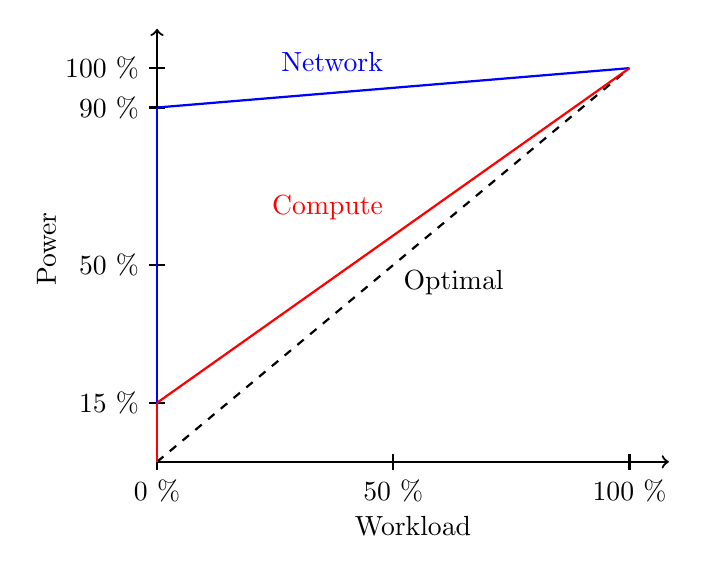
\begin{tikzpicture}

		% --- Grid/Axes Setup ---
		\draw[->, thick] (0,0) -- (6.5,0) node[below=16pt, pos=0.5] {Workload};
		\draw[->, thick] (0,0) -- (0,5.5) node[left=40pt, rotate=90, pos=0.6] {Power};

		% --- Tick Marks ---
		% X-axis
		\foreach \x/\label in {0/0 \%, 3/50 \%, 6/100 \%} {
			\draw[thick] (\x, -0.1) -- (\x, 0.1);
			\node[below=3pt] at (\x, 0) {\label};
		}
		% Y-axis
		\foreach \y/\label in {0.75/15 \%, 2.5/50 \%, 5/100 \%, 4.5/90 \%} {
			\draw[thick] (-0.1, \y) -- (0.1, \y);
			\node[left=3pt] at (0, \y) {\label};
		}

		% --- The Curves ---
		
		% Optimal Line (Dashed)
		\draw[dashed, thick] (0,0) -- (6,5) node[midway, below right, yshift=2pt] {Optimal};

		% network Line 
		\draw[thick, color=blue] (0,0) -- (0,4.5);
		\draw[thick, color=blue] (0,4.5) -- (6,5) node[midway, above left, yshift=2pt] {Network};

		% compute Line 
		\draw[thick, color=red] (0,0) -- (0,0.75);
		\draw[thick, color=red] (0,0.75) -- (6,5) node[midway, above left, yshift=2pt] {Compute};

	\end{tikzpicture}
	\caption{Power Proportionality relations.}\label{fig:GraphPowProp}
\end{figure}


Regarding the power drawn by each side during an iteration the following considerations are taken into account :
\\On the \textit{computing side}, the maximum power is \qty{500}{\watt} per host (\qty{400}{\watt} for the GPU and \qty{100}{\watt} for CPUs, RAM, storage and fans). The power proportionality is 85\% \cite{ComputePowProp} resulting in an idle power of \qty{75}{\watt}. The power proportionality of the computing side is represented in red in Figure \ref{fig:GraphPowProp}.
\\On the \textit{networking side}, the article model Switches, NICs and transceivers with 10\% power proportionality, resulting in 90\% of the max power drawn idling, represented in blue in Figure \ref{fig:GraphPowProp}.
A switch has a \qty{750}{\watt} maximum power resulting in \qty{675}{\watt} in idle power (90\% of the max power).
This illustrates the issue of low power proportionality, as even when idling, due to the lack of energy-saving mechanism at low workloads, switches consume nearly the same power when working or idling.     
The power draw of NICs and transceivers with respect to the considered bandwidth is featured in Table \ref{tab:PowNicTrans}, missing values are extrapolated linearly from the last available value.
Again, as for the workload model, the linear extrapolation underestimates by overlooking overheads due to scaling.     


\begin{table}[t]
	\caption{Maximum power values for network components.}\label{tab:PowNicTrans}
	\centering
		\begin{tabular}[c]{cccccc}
			\toprule
			\textbf{Bandwidth(Gbps)} & \textbf{100} & \textbf{200} & \textbf{400} & \textbf{800} & \textbf{1600} \\

			\hline
			\textbf{NIC} & 8.6 & 16.7 & 25.4 & 38.6* & 58.8*\\ 
			\hline

			\textbf{transceiver} & 4 & 6.5 & 10 & 16.5 & 27.2*\\ 
			\bottomrule
		\end{tabular}
		\caption{\hspace{4.5cm} * linearly extrapolated value}
\end{table}

To be able to calculate the overall power drawn, it is necessary to know the number of switches, NICs, and transceivers.
The number of switches in the model is calculated from formulas \cite{Demy} considering a fat-tree topology and is interpolated if the number of hosts is between what a certain number of stages (layers) could support.
The number of NICs corresponds to the number of hosts, \textit{i.e.} 15k.
The transceivers to consider in the model are those connecting switches together, as transceivers between end hosts and switches are electrical, which have a negligible impact on power. 


This interpolation of the number of switches is not precisely disclosed in the paper, making the derivation of the number of switches difficult.
Moreover, as the number of switches is hard to derive, it implies that the number of transceivers between switches is also difficult to derive.

An, initial and uninformed, attempt at reproducing the paper's result is presented in Appendix \ref{app:attempt}. 
Though the paper does not fully disclose the underlying computation necessary, contacting them made them realise that the GitHub repository \cite{githubeNetPowProp} containing all the calculations and figures creation was in private.  

Once the GitHub repository was set to public, the underlying computation of the number of switches became clear.
First, the number of ports $N_\textnormal{port}$  is computed as the integer division of the total switch bandwidth $Sw_\textnormal{Bw}$ and individual port bandwidth $Port_\textnormal{Bw}$, considering the switch bandwidth is evenly distributed on every port.
\begin{equation}
	N_\textnormal{port} = Sw_\textnormal{Bw} // Port_\textnormal{Bw}
\end{equation}

Then, the number of switches $N_\textnormal{Sw}$ is computed using the number of layer $L$ :
\begin{equation}
L = \frac{log(N_\textnormal{hosts}/2)}{log(N_\textnormal{port}/2)}
\end{equation}
\begin{equation}
N_\textnormal{Sw} = (2L - 1) \cdot (\frac{N_\textnormal{port}}{2})^{L-1}
\end{equation}

Finally, the number of transceivers $N_\textnormal{trx}$ is computed by removing the hosts connections from the total number of connections:
\begin{equation}
N_\textnormal{trx} = N_\textnormal{Sw} \cdot N_\textnormal{port} - N_\textnormal{hosts}
\end{equation}


\subsection{Impact of Poor Power Proportionality}\label{sec:impact}
The power footprint of the networking and computing hardware for the examined ML cluster calculated by the article depending on the phase is presented in Figure \ref{fig:PowFootprint}.   

As expected, computing hardware has the largest footprint during the computation phase.
However, an interesting observation can be made regarding the network power footprint in absolute terms (Fig. \ref{fig:PowAbs}) from the article.
Due to the low power proportionality of the network, its footprint stays relatively constant across both phases, \textit{i.e.} the absolute power draw is only slightly reduced when idling. 
Moreover, its efficiency computed as $\frac{\textnormal{useful power}}{\textnormal{total power}}$ for an iteration reaches as low as 11\%.
This is due to the combination of the low power proportionality making the network waste a considerable amount of power while idling and its high idling ratio (90\%).
Furthermore, as the network power footprint accounts for an average of 12\% of the total cluster's energy consumption, the question of increasing the network power proportionality is relevant to explore.  

Investigating the power-savings resulting from an increase in network power proportionality the article \cite{NetPowProp} finds interesting results.\\
At the considered bandwidth of the cluster, with 50\% (resp. 85\%) power proportionality the power-savings would be around 5\% (resp. 9\%) of the total cluster power.
Those results are significant, as even 5\% of reduction, due to its scale, a considerable amount of power.


\begin{figure}[t]
		\centering
		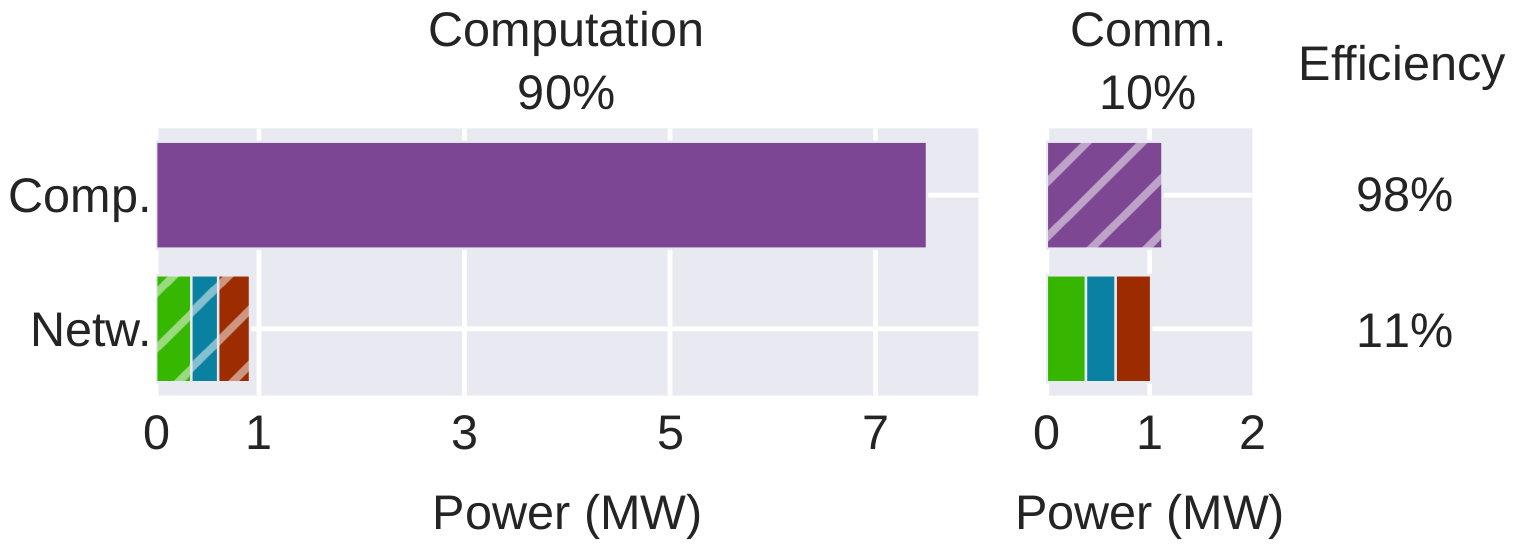
\includegraphics[width=0.95\columnwidth]{figures/PowerFootPrintComp.png}
	\caption{Power footprint with an iteration standpoint and efficiency perspective.}\label{fig:PowAbs}
\end{figure}


\begin{figure*}[ht]
	\centering

	\subfloat{
		\centering

		\begin{tikzpicture}[
			square/.style={minimum size=0.6cm, inner sep=0pt},
			label_text/.style={font=\sffamily\Large, anchor=west, xshift=0.3cm}]
			% --- First Column ---
			\node[square, fill=Fuchsia, scale=0.8] (s1) {};
			\node[label_text] at (s1.east) {GPU and Servers};
			\node[square, fill=BrickRed, scale=0.8, below=0.3cm of s1] (s2) {};
			\node[label_text] at (s2.east) {Transceivers};

			% --- Second Column ---
			% Positioned 4cm to the right of the first column
			\node[square, fill=ForestGreen, scale=0.8, right=5cm of s1] (s3) {};
			\node[label_text] at (s3.east) {NICs};

			\node[square, fill=Turquoise, scale=0.8, below=0.3cm of s3] (s4) {};
			\node[label_text] at (s4.east) {Switches};


		\end{tikzpicture}	
	}
	\hfil

	\subfloat[Computation phase]{
		\centering
		\donutchart[rotate=90]{89.1/Fuchsia/GPU and Servers, 3.1/Turquoise/Switchs, 3.7/BrickRed/Transceivers, 4.1/ForestGreen/NICs}{8.4 MW}
	}
	\subfloat[Communication phase]{
		\centering
		\donutchart[rotate=90]{52.6/Fuchsia/GPU and Servers, 13.5/Turquoise/Switchs, 16.1/BrickRed/Transceivers, 17.8/ForestGreen/NICs}{2.1 MW}
	}
	\caption{Power footprint of the cluster calculated by the authors.}\label{fig:PowFootprint}
\end{figure*}



\subsection{Increasing power proportionality in the network}\label{sec:PowSol}
This section focuses on increasing the network power proportionality by exploring implemented optimisations from computing hardware.
These optimisations can be separated in two categories, static optimisation, \textit{i.e.} adjusting hardware to have the lowest power draw at zero load and dynamic optimisation, \textit{i.e.} scaling power demand with the load.

\textbf{Static Opt.1: Exposing power knobs}\\
\textit{From computing hardware} : Users are able with gating mechanisms to power off unnecessary components such as PCIe slots or memory banks.
Frequently, these parameters are also applicable to OS features and are packaged under predefined configurations, \textit{e.g.} CPU C-states. \\
\textit{To networking hardware} : Such configurations could also be applied to networking hardware.
For example, a Layer 3 switch used only for L2 capabilities isn't required to have routing tables which could then be turned off.\\
\textit{Challenges} : Just as CPU manufacturer, network hardware manufacturer reluctant to giving too much information about the components and architecture. 
Thus, finding a balance between secrecy and modularity should be addressed to enable users to have as much control as possible without exposing hardware details.


\textbf{Static Opt.2: Scheduling network jobs}
\\\textit{From computing hardware} : In ML clusters, job schedulers enable traffic to be directed to a restrained set of servers to free other servers from running at full pace or completely.   
\\\textit{To computing hardware} : Similar mechanism could be introduced by using Optical Circuit Switches (OCSs). Such switches avoid the optical - electrical - optical conversion and work directly with optical signals. 
As those switches use (physical) mirrors, their reconfiguration speed is slow.
Nevertheless, in the case of an ML cluster, reconfigurations follow the ML training job which may last for hours or days.
This permits the use of OCS in such environment. 
\\\textit{Challenges} : The placement of such OCS in the cluster topology could leverage the cluster's job schedules.
Though the number and placement of those switches is an interesting question with an underlying trade-off between energy savings and reaction time. 


\textbf{Dynamic Opt.1: Rate adaptation}
\\\textit{From computing hardware} : A classic rate adaptation implementation is the dynamic voltage and frequency scaling (DVFS), which can reduce the clock speed of cores depending on the load.
\\\textit{To networking hardware} : DVFS can be applied in a router's control plane, but wouldn't save much energy as it only consumes a fraction of the router's power footprint.
However, applying such concept to the data plane by, for example, reducing the ASIC's clock frequency or turning off an interface's SerDes component, could yield significant energy savings.
Moreover, it could also be applied to network interface cards and transceivers as their power footprint share isn't negligible.
\\\textit{Challenges} : Rate adaptation of the ASIC's clock isn't perfect as it would require ASIC's pipelines to be independent.
Though, this would need an ASIC redesign which is a substantial change. 


\textbf{Dynamic Opt.2: Turning off pipelines}
\\\textit{From computing hardware} : Depending on the load, CPUs are capable of turning off some of their cores. 
\\\textit{To networking hardware} : Turning off pipelines, which are the physical unit in charge of packet arrival and departure, would significantly reduce power footprint. 
\\\textit{Challenges} : In actual ASICs, pipelines are tied to a subset of ports, which makes turning off entire pipelines more complex, as it would simply turn off all the ports it's tied to.
A solution could be to introduce an (optical) circuit switch in front of a switch's ports to map packets arrival in the active pipelines.
Though a possible solution, it introduces latency in the system, as the circuit switch might not consume much but would need buffering, implying need to decode and re-encode the packet, which consumes energy.

\subsection{Conclusion}
In this section, we focused on the impact of low proportionality of state-of-the-art networking hardware in the context of a machine learning cluster. 
Modeling the use of one pod of this cluster (Section \ref{sec:PowMod}), was initially complicated due to the lack of transparency regarding topology interpolation.
These complications inspired an attempt (in Appendix \ref{app:attempt}) to reproduce the article's results yielding higher total power consumption.
However, contacting the authors solved the problem as they changed their GitHub\cite{githubeNetPowProp} repository's visibility to public.  

The authors find that the network accounts for on average 12\% of the total cluster power consumption and argue that improving network power proportionality could lead to power-savings ranging from 5\% up to 9\%.
In the attempt, the network accounts for on average 14\%, leading to even higher power savings.
The power efficiency found in the article, due to the poor power proportionality and high idling time, reaches an appallingly low 11\%.
These results represent, in the context of million-watts power consumption of the cluster, a considerable amount of wasted energy.

In the context of green networking, such amounts represent non-negligible insights and should be a concern to investigate further, especially in the case of machine learning clusters or data center due to their recent growth in number, large scale and low communication rate.  

To investigate possible solutions, improvements regarding the power proportionality of network devices are explored from static and dynamic viewpoints by taking inspirations from the computing hardware strategies.
Even though such improvements would likely require ASIC and software changes, as demonstrated by the modeling, they are worth investigating further and should interest network hardware manufacturers.  


